%\clearpage





\section{Open question}
Now we would like to address the following question: "It is possible to classify months characterized by government crisis, only by using graph features?".\\
First, it's important to define what we are searching for. Italian politics is characterized by strong instability, the expected life for a government is 414 days, which becomes 380 days not considering the \textit{'sede vacante'} days, the period between the fall of a government and the start of a new one. Keeping this in mind, we tried to exploit the differences between the different months, using extracted data, to learn whether the voting patterns and the networks built from them can be used as predictors for an imminent crisis, and a consequent fall in the government.\\

The first problem encountered in this analysis was to precisely define how to label our month as a crisis (class 1) or not a crisis (class 0). 
The information regarding the month when a government officially ended is easily retrieved. However, we thought that the period of political instability could not be restricted to only that month.

That's why we decided to label it as '1' both the month before the fall of the government and the month after. We recognize that this was an arbitrary definition, and this would deserve a more in-depth study.\\
In the end we had $15\%$ of the entire dataset labeled as 1, the rest labeled as 0.\\

\begin{figure*}[h]
  \centering
  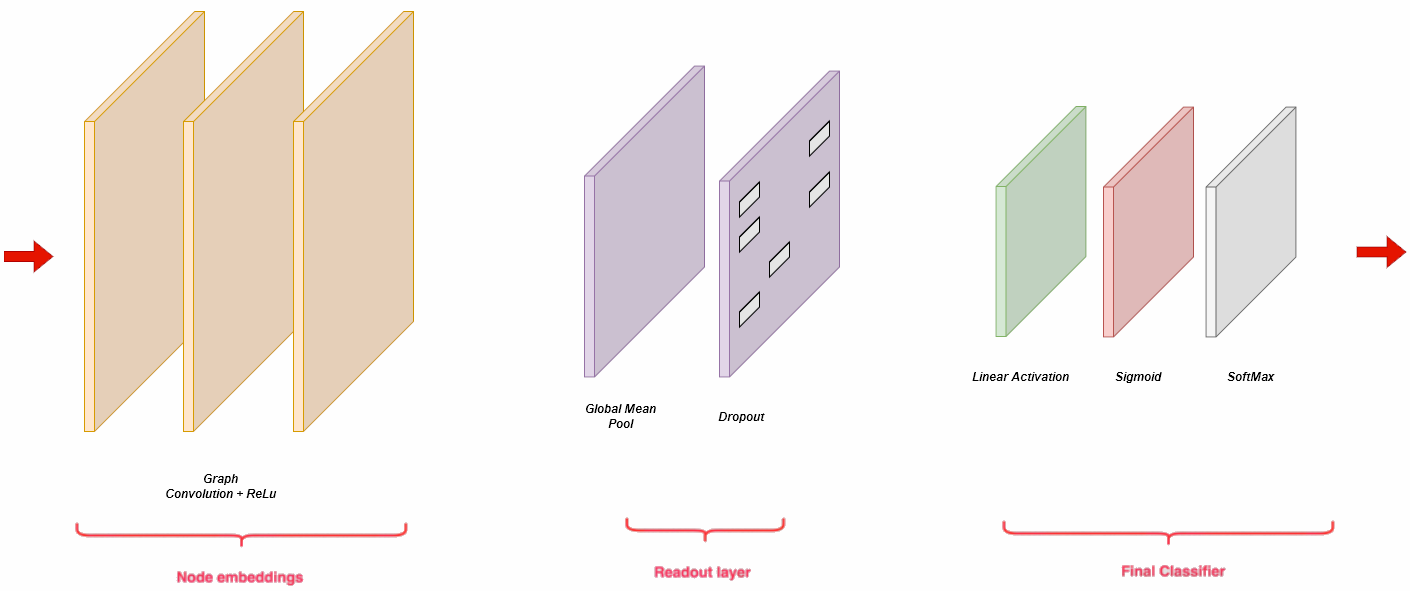
\includegraphics[width=0.9\linewidth]{img/nn scheme.png}
  \caption{Scheme of the GNN used for our graph classification task. First, we do a convolution, based on the adjacency matrix, in order to embed every node of the graphs. Then we use a global mean pool layer to aggregate node embeddings into a single graph embedding. Finally, we train a classifier to complete the task.}
  \label{fig:nn}
\end{figure*}

\subsection{Graph Neural Network}

Our main task was a binary classification one, we decided to build a Graph Neural Network (GNN) and classify each graph based on the information embedded in the structure.\\
The idea is to embed graphs based on their structural properties, in such a way so that they are linearly separable.\\

The first thing we did was prepare the dataset for the classification task.\\
To create a Graph dataset we followed the official documentation\footnote{\url{https://pytorch-geometric.readthedocs.io/en/latest/tutorial/create_dataset.html}} of \textit{Pythorch Geometric}.

After defining the labels for the graphs, we split the data into train and test, using a classical train-test split with stratification on the target variable. For the model evaluation, we trained our network using the binary categorical cross-entropy as loss function.\\
As input features, we used the adjacency matrix of the graph, automatically extracted by the \textit{PyG} library, and, for each node, we extracted some metrics to help the classification model in the task. In particular we used:
\begin{itemize}
    \item Node degree 
    \item Betweenness Centrality
    \item Closeness Centrality
    \item PageRank
    \item Eigenvector Centrality
\end{itemize}

Then we defined the structure of the GNN. Our model learns to classify graphs using three main steps (schematized in figure \ref{fig:nn}):
\begin{enumerate}
    \item Embed nodes using several rounds of message passing. In this case, we use three convolutions layers, each of which is followed by a ReLu layer.
    \item Aggregate these node embeddings into a single graph embedding (called readout layer). The average of node embedding is used (global mean pool).
    \item Train a classifier based on graph embedding. We decided to add a Dropout layer, setting p = 0.5, then a Sigmoid layer, and a final Softmax layer to extract the probability associated with each class.
\end{enumerate}
We divided the train set in batches, and start the training of our models, adding a regularization term to avoid overfitting. To avoid overtraining our model, we split the train set into train and validation, and, during training, the model is evaluated on a holdout validation set after each epoch. If the performance of the model on the validation set starts to degrade, then the training process is stopped. We defined a 'patience' parameter with a value of $15$. \\

After the first training session, the performance wasn't exciting, the loss in training was halved, but the accuracy in the testing phase was $0.25$. However, this value has not much meaning, since our classifier always predicts the same label.\\

We note that our dataset has a class imbalance: this may represent a problem because the model is unable to learn meaningful features from the data and predicts the majority class all the time.
 The optimizer finds a local minimum for the loss, corresponding to always predicting the class which is dominant in the dataset.\\

We decided to modify the loss function, accounting for the imbalanced scenario and weighting the classes based on the sample size for each class. Despite all our efforts, the performance didn't change. Our model did not recognize different patterns between crisis months and 'normal' months.\\


Another approach to solving the problem can be data augmentation: a first idea could be oversampling the minority class or undersampling the majority class.
 Another possibility is to synthetically create data of unbalanced classes which are similar to the existing ones.\\
We tried to undersample the majority class, creating a dataset with an equal number of 'crisis' and 'normal' months. However, also, in this case, the network could not learn from the data, predicting always 'crisis' or always 'normal'.\\

At this point we believe that a more fundamental problem could be happening: the graph structure and the node features we are considering are not informative enough. It can be the case that there are some other features that better capture the instability of the political scenario. Or simply it can be that there is not a significant correlation between the voting behaviors of Deputies and the government crisis.\\

One aspect of our classification approach is that it does not consider the previous history of the network, but tries to predict if a month is "of crisis" or not, just by considering the features of that specific month. Approaches that also consider the history of the network should be investigated, for example, a Recurrent Graph Neural network could be optimal for this scope.\\

Other strategies can be pursued as well, one involves the study of how can we define a government crisis, and how to convert the information in network structure, using the partisan discipline to add insights into the voting behavior. Moreover, one can focus on why the model fails to recognize different labels and, using explainability frameworks, discover what feature can contribute to the final classification.


